\section{La ricerca}

html.it è un autentico portale più che un sito web. Consiste di decine, forse centinaia di articoli e guide, si sviluppa su diversi rami e raccoglie un'infinità di informazione. Quando si ha a che fare con siti web di questa portata è essenziale dotare il medesimo di un sistema di \textbf{ricerca interna} che sia il più eccellente possibile e soprattutto che sia simile al modo in cui l'utente è solitamente abituato ad effettuare la ricerca.

html.it utilizza un tool di google per effettuare ricerche interne al sito. Questa è una soluzione veloce, a costo zero ed efficace in quanto utilizza il motore di ricerca google che è indubbiamente il più utilizzato nel web. La barra di ricerca è molto ben visibile e può contenere un buon numero di caratteri (>30). Proviamo ad effettuare una ricerca e vediamo i risultati ottenuti. Cerchiamo ad esempio il termine ``usabilità'':

\begin{figure}[H]
\centering
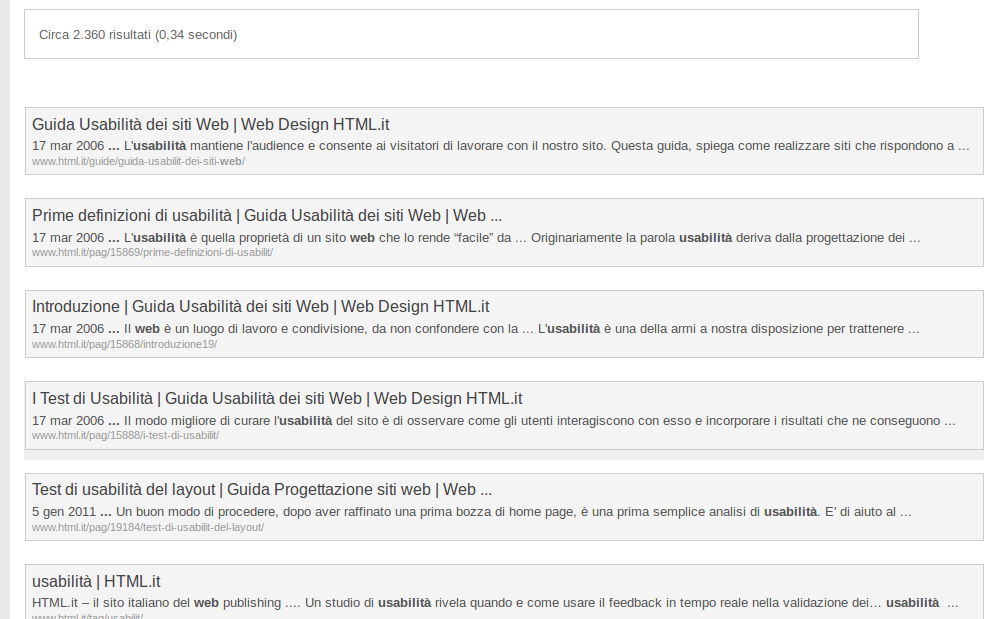
\includegraphics[width=120mm]{images/search.png}
\caption{I risultati di una ricerca}
\end{figure}

Come possiamo vedere la ricerca produce tutti risultati interni al sito in modo paginato visualizzandoli a lista e riesce a rispondere in modo efficiente alla nostra richiesta. Questo approccio è ottimo, purchè progettato per funzionare su bassa scala. Se infatti l'utente riusa la ricerca interna fatta precedentemente all'esterno significa che il motore di ricerca non gli ha fornito l'informazione cercata e quindi la ricerca fatta allo stesso modo produrrà il medesimo risultato. Inoltre i motori di ricerca troncano il 50\% delle indicizzazioni, quindi verrà fatto anche in locale, con perdita della metà delle informazione.

In conclusione la soluzione adottata è buona, fornisce quanto richiesto ma non è la soluzione ottima. L'idea migliore sarebbe quella di sviluppare un motore di ricerca interno progettato dagli sviluppatori del sito in modo che effettui ricerche in base alla struttura del sito. Ciò chiaramente comporta un costo in termini di tempi e risorse da impiegare per la progettazione e la codifica. Cionondimeno sarebbe sicuramente una buona feature da sviluppare in futuro.


